%%%%%%%%%%%%%%%%%%%%%%%%%%
% MSc Project Background Report Template
% Guy Brown
% University of Sheffield
% 20th Feb 2015
%%%%%%%%%%%%%%%%%%%%%%%%%%

% This version of the template uses standard latex fonts

\documentclass[11pt,oneside]{book}
\usepackage[margin=1.2in]{geometry}
\usepackage{setspace}
\usepackage[toc,page]{appendix}
\usepackage[none]{hyphenat} % turn hyphenation off by default
\usepackage{graphicx}
\usepackage{color}
\usepackage{url}
\usepackage{amsmath}
\usepackage{listings}
\usepackage{algorithm}
\usepackage{algorithmic}
\usepackage{subfig}
\usepackage{hyperref}
\usepackage{dirtytalk}

\hypersetup{
    colorlinks,
    citecolor=black,
    filecolor=black,
    linkcolor=black,
    urlcolor=black
}


\begin{document}

\frontmatter

\begin{titlepage}

% You need to edit the details here

\begin{center}
{\LARGE University of Sheffield}\\[1.5cm]
\linespread{1.2}\huge {\bfseries Spider Animation}\\[1.5cm]
\linespread{1}

\includegraphics[width=5cm]{images/tuoslogo.png}\\[1cm]
{\Large Wuhao Wei}\\[1cm]
{\large \emph{Supervisor:} Steve Maddock}\\[1cm]
\large A report submitted in fulfilment of the requirements\\ for the degree of MSc in Advanced Computer Science\\[0.3cm] 
\textit{in the}\\[0.3cm]
Department of Computer Science\\[2cm]
\today
\end{center}

\end{titlepage}

% -------------------------------------------------------------------
% Declaration
% -------------------------------------------------------------------

\newpage
\chapter*{\Large Declaration}

\setstretch{1.1} % set the line spacing differently if you wish, but this looks good to me. 

All sentences or passages quoted in this report from other people's work have been specifically acknowledged by clear cross-referencing to author, work and page(s). Any illustrations that are not the work of the author of this report have been used with the explicit permission of the originator and are specifically acknowledged. I understand that failure to do this amounts to plagiarism and will be considered grounds for failure in this project and the degree examination as a whole.
 
\noindent Name:\\[1mm]
\rule[1em]{25em}{0.5pt}

\noindent Signature:\\[1mm]
\rule[1em]{25em}{0.5pt}

\noindent Date:\\[1mm]
\rule[1em]{25em}{0.5pt}

% -------------------------------------------------------------------
% Abstract
% -------------------------------------------------------------------

\chapter*{\Large \center Abstract}
Previous work on arthropod animation can be divided into two main categories: data driven approach and physical modeling approach. The locomotion of various arthropods has been extensively studied in biology and robotics. A simulation of arthropod could be used in various meaningful scenarios such as animation movies, computer games, etc.



The aim of the project is to develop realistic spider animation that could be observed closely using the Oculus Rift. The purpose of this report is to review general animation techniques, knowledge for simulating an arthropod and finally come up with possible solutions for spider animation. The general animation adopted for the project is procedural animation. Two main approaches proposed to control the animation are: scene graph and hierarchy with rigging and skinning.




% -------------------------------------------------------------------
% TOC etc
% -------------------------------------------------------------------

\tableofcontents
\listoffigures
\listoftables

\setstretch{1.1} 

\mainmatter

%%% Local Variables:
%%% mode: latex
%%% TeX-master: "..\main_standard"
%%% End:

\chapter{Introduction}
\section{Aims and objectives}
The main aim of the project is to develop realistic spider animation.
A subsidiary aim is to enable people to be immersed in the animation by using the Oculus Rift. 
The result of the spider animation does not have to exactly follow the constraints of biology or physics, 
but should produce an animation which could deceive people to believe that it is real. 

The project will be divided into two main parts: animation and rendering. 

The most important part of the animation is the locomotion behavior which mainly handles 
the way in which the spider makes a step. 

There are three main general methods used to achieve this: keyframe animation, procedural animation and physical simulation. Usually, a keyframe method cannot tackle the task easily, since the keyframe animation mainly injects rules of attributes into a function of time.  One obvious advantage of physical animation compared to procedural method is that it provides clues to control a spider robot while the main aim of the project is to develop animation. As a result of this, the project will adopt a procedural method that mainly involves combining rules learned from biology or observation with kinematic animation.  

Since the project will adopt skeletal animation, it is required that a model of the spider is built before trying to animate it. Figure  \ref{fig:realSpider} is an image of a real wolf spider and Figure \ref{fig:spiderModel} is a similar model to the real wolf spider.


\begin{figure}[ht!]
\centering
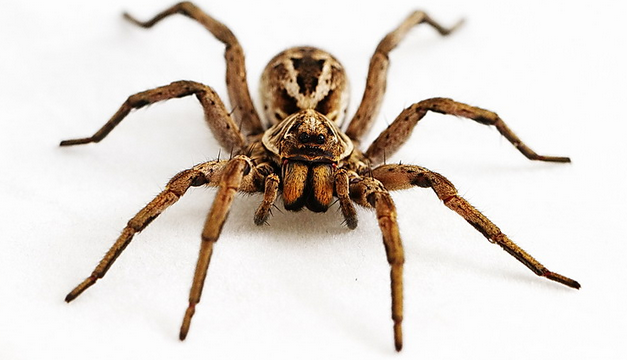
\includegraphics[width=14cm]{figures/realSpider.png}
\caption{A real wolf spider. \protect\footnotemark}
\label{fig:realSpider}
\end{figure}

\footnotetext{\url{http://photos.beilby.com/index.php?showimage=1117}. Gary Beilby. asking permission ...}

\begin{figure}[ht!]
\centering
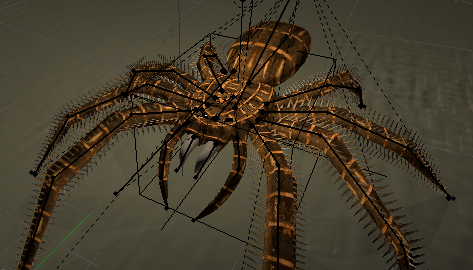
\includegraphics[width=14cm]{figures/spiderModel.png}
\caption{A wolf spider model  \protect\footnotemark}
\label{fig:spiderModel}
\end{figure}
\footnotetext{\url{http://www.blendswap.com/blends/view/26798}. DennisH2010. }

\cite{thesis} is a research about arthropod animation which implemented a hybrid approach. This includes procedural and physical approaches. The work of \cite{thesis} is based on the three locomotion layers proposed in \cite{steering}. \cite{steering} has divided the locomotion animation into three main parts: action selection, steering behavior and locomotion behavior. Thus the main objectives of the animation part is to implement the steering and locomotion behavior layers in \cite{steering}.

While the rendering part is also important due to the aim of observing the animation closely. A general texture mapping is not sufficient for the task as the close observation requires a considerable level of detail(e.g. fur of the spider). There are two methods specifically for rendering fur of an arthropod. These are side-view texture mapping and fins and shells techniques\cite{fur}. However, due to the limited time of the project, initially only polygon meshes or simple texture mapping will be considered.
The Oculus Rift is a virtual reality headset developed by Oculus VR. It enables users to seamlessly look around the virtual world. It tracks every little movement of users' head to create a natural experience \cite{rift1}. Figure \ref{fig:rift} is an image of device Oculus Rift 2.



\begin{figure}[ht!]
\centering
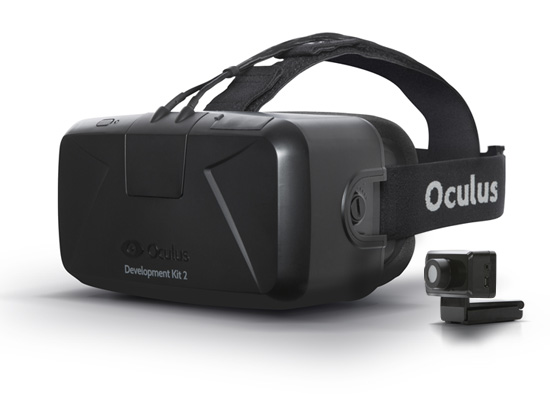
\includegraphics[height=8cm]{figures/rift.jpg}
\caption{Oculus Rift 2. \protect\footnotemark}
\label{fig:rift}
\end{figure}
\footnotetext{\url{https://www.oculus.com/rift/}. Oculus Rift Official Website.}

\section{Overview of the report}
The remaining report is structured as follows: 
\begin{itemize}
  \item \textbf{Chapter 2} will review previous research and techniques relevant to this project. This chapter will also discuss general animation techniques. Then animation and rendering techniques specifically for arthropods will be covered.
  \item \textbf{Chapter 3} will analyze the aims of the project and divide the project into manageable subtasks. Evaluation criteria is also included in this chapter. 
  \item \textbf{Chapter 4} will give a plan about how the project will be done based on possible solutions proposed in Chapter 3. Risk analysis and possible countermeasures will also be included in this chapter.
  \item \textbf{Chapter 5} will draw a conclusion that briefly summarizes work done for the background report and the future work according to the plan proposed in Chapter 4.
\end{itemize}



% !TEX root = ../main_standard.tex
\chapter{Literature Review}
In this chapter, previous research and techniques relevant to the
project are reviewed. The first part of the chapter basically describes
the general animation techniques such as key frame animation,
procedural animation, kinematic animation and physical animation. The
fundamentals of animation such as how to represent an object and
manipulate these objects are also included in this part. The second
part mainly focus on rendering techniques and animation techniques
specifically for the arthropods.

% section aaa (end)
\section{Understanding of a spider} 
Spiders belong to a class of animals called "arachnids", which also includes mites, ticks, scorpions and pseudoscorpions\footnote{\url{http://www.kidzone.ws/lw/spiders/facts01.htm}}. Arachnids are a class of joint-legged invertebrate animals called arthropods which also include insects and crustaceans(lobster, crabs, etc)\footnote{\url{https://en.wikipedia.org/wiki/Arthropod}}. A spider is not an insect and the most obvious difference is the insects have six legs and three main body parts while the spider has eight legs and two main body parts. 

The most visible parts of a spider which marked blue in figure \ref{fig:partsOfSpider} are abdomen, cephalothorax and legs. The less visible parts of a spider which marked red in figure \ref{fig:partsOfSpider} are pedipalp, chelicera and eyes. 

The spider in \ref{fig:closeViewSpider} is a wolf spider which has six eyes(most spiders have eight eyes) and most parts of it are covered with many hairs. A spider does not have skeletons or bones. Instead they have a hard outer shell called an "exoskeleton". The "exoskeleton" does not grow with the spider, so when a spider grows, it has to molt.


\begin{figure}[ht!]
\centering
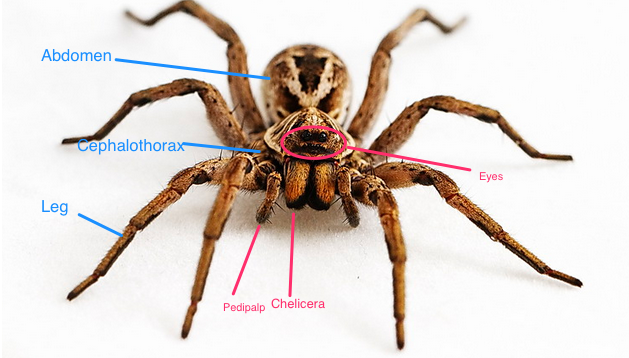
\includegraphics[width=14cm]{figures/partsOfSpider.png}
\caption{Visible body parts of a spider. \protect\footnotemark}
\label{fig:partsOfSpider}
\end{figure}
\footnotetext{\url{http://photos.beilby.com/index.php?showimage=1117}. Gary Beilby. Permission from author.}


\begin{figure}[ht!]
\centering
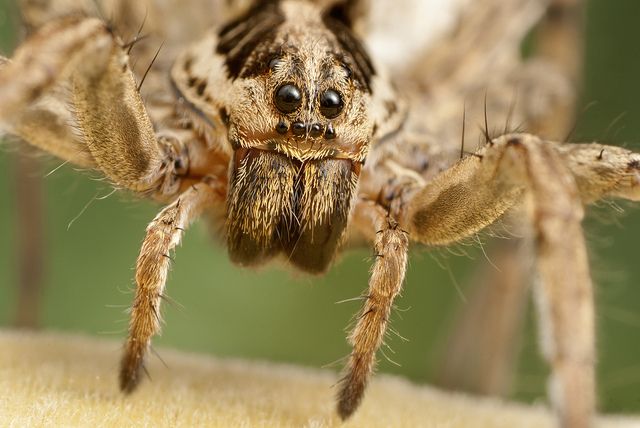
\includegraphics[width=14cm]{figures/wolfspidereyes.jpg}
\caption{Close view of a wolf spider. \protect\footnotemark}
\label{fig:closeViewSpider}
\end{figure}
\footnotetext{\url{http://www.kidzone.ws/lw/spiders/facts02.htm}. photo by Anxo Resúa. licensed under CC BY-SA 2.0.}


The next section will discuss computer graphics techniques for modelling a spider. Spider simulation will be discussed in \ref{sec:arthropod_simulation}.


\section{Representing an object} 
There are many alternative representations of an object in computer graphics, such as polygons, parametric patches, constructive solid geometry, etc. Among these representations, the most popular method is using polygonal facets, usually a mesh of triangles which referred as a Boundary representation \cite{alan3D}.This section will discuss how to use polygon meshes to represent an object and how to manipulate them. There are three subsections in this section. In the first subsection, a simple cube model using face-vertex will be introduced. The second subsection will generally describe the control techniques(rigging and skinning) for more complex mesh models such as a human model. In the final subsection, a robot model made of basic geometric shapes such as sphere and cylinder will be built with the help of scene graph. How to manipulate the robots into different postures with scene graph will also be included in this subsection. 



\subsection{A simple mesh model} 
Polygon meshes also could be represented in various ways by using different methods to store the vertex, edge and data. 
One most widely used is face-vertex meshes\cite{facevertex}.
In face-vertex meshes, an object is represented as a set of faces and
a set of vertices. Face-vertex meshes allow both explicit lookup of
the vertices of a face and the faces surrounding a vertex. Figure
\ref{fig:graph1} is a cube example as a face-vertex mesh. Since in
this example, every face is represented in a triangle, each face has
exactly three vertices. However, it is easily seen that not every
vertex has same number of faces(e.g., v0 has 5 faces, v8 has 4
faces). 
\begin{figure}[ht!]
\centering
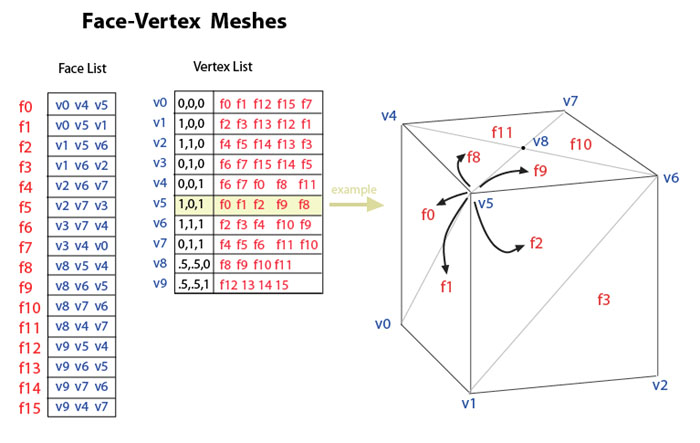
\includegraphics[width=13cm]{figures/figure1.jpg}
\caption{Face-Vertex Meshes \protect\cite{fv}}
\label{fig:graph1}
\end{figure}
The advantages of face-vertex meshes is that it is easy to traverse all structures. Moreover, locating neighboring faces and vertices is constant time because both faces and vertices are explicit. However, it is not same case for locating face given another face because the edge information is implicit. In rendering process, the face list usually transmitted into the GPU as a set of indices and each vertex usually contain three properties: position, normal and color. The advantage of this is when the shape is changed, only the vertex data need resending without updating the face connectivity.
Despite the popularity and simplicity of polygon meshes, there are difficulties in changing the shape in animation. First, moving polygon mesh vertices will disrupt the where a shape has been converted into polygons with some degree of accuracy. Second, altering a large part of an object which may involve moving many elements at the same time. Third, the level of details should also be considered when rendering from different distances \cite{alan3D}. 
\subsection{A complex surface mesh model}
The left part of figure \ref{fig:rigging} is a complex human mesh model. It is easier to manipulate the complex mesh model in a hierarchical structure.
\begin{figure}[ht!]
\centering
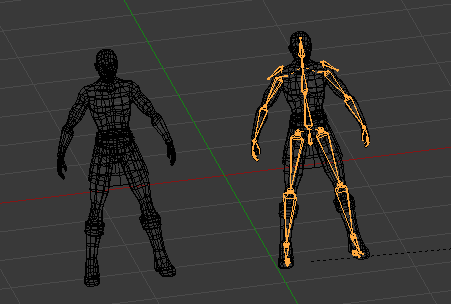
\includegraphics[height=8cm]{figures/rigging.png}
\caption{A complex human mesh and rigging \protect\cite{shaolinpic}}
\label{fig:rigging}
\end{figure}
Usually to animate or pose a complex articulated structure, a set of
bones or skeletons are added such as the right part in figure \ref{fig:rigging}.  As a result, when we want to make the angle between 
upper arm and lower arm as 60 degrees, we could make the angle of the bones as 60 degrees.
This process is called rigging which
usually includes linking the bones in a hierarchy,
setting constraints on the bones' movement(usually degrees of freedom
of the joints), and set up controls such
as inverse kinematics and forward kinematics.
There are also many automatic rigging techniques which saves lots of
artists' time. \cite{Rigging1} implemented a system can automatically rig and skin, in which the main method adopted is to calculate the bone iteratively based on assuption of weight-like parameters.  \cite{Rigging2}  implemented a more advanced system by adopting an example-based rigging approach where the skeleton is more compatible with most existing popular animation software.
\subsubsection{Skinning}
Skinning is to bind a skin to the skeleton which means that every
vertex of the continuous skin mesh is attached to a joint. As a
result, the skin vertices are moved when the skeleton is moved.
A basic skinning approach is rigid skinning where the relative
position of the vertex in the local joint frame does not change. It is simple but has the disadvantage
of large distortions at bends. Vertex blending is another approach
which tackles this problem but has the skin collapse problem
\cite{skinning1}. \cite{skinning2} implemented an approach which could
automatically skin deformable mesh animations with no need for
specifying skeletons.
\subsection{A complex object built from pieces}
An alternative way to build an object is to use pieces rather than a single complex mesh. As an example, we will consider building a robot from pieces. The most obvious way to do it is directly put the
pieces in certain position. However, problems come when we want to make
the robot pose in certain gestures. Because it is hard to calculate the
final position and orientation of some parts of it such as the finger
of the robot. It will be
much more simple if the relationship of different parts could be
taken into consideration(e.g., when the arm rotates around shoulder,
the finger will translate and rotate accordingly). 
A scene graph is a general data structure which arranges the logical representation of a
graphical scene. 
It is usually represented in a collection of nodes in
a graph or tree structure. It also could be used to structure the parts of a complex object made of pieces. For example, Figure \ref{fig:graph3}  is a simple robot example and
its scene graph.  The nodes can also be grouped into a compound object(e.g. the left shoulder and
all its child could be grouped as left arm.) that can be
transformed, selected, etc. as easily as a single object.   
An operation on a parent node automatically
propagates its effect to all its child nodes. If the upper arm rotates around the shoulder, all its
child nodes(e.g., elbow, lower arm etc.) will be affected. Figure
\ref{fig:scenegraph2} is the robot and its scene graph after adding two
rotation R1 and R2. It is easily seen the advantages that only by
rotating the two upper arms around their shoulders, all its child
nodes such as elbow, lower arms, palm and fingers will move
automatically without specific transformations on these nodes.
\begin{figure}[ht!]
\centering
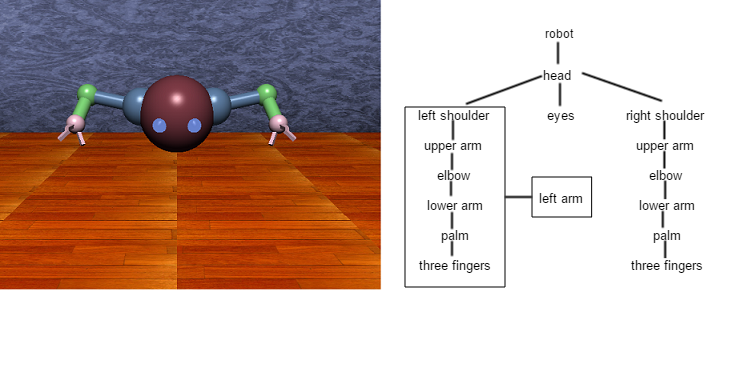
\includegraphics[width=12cm,height=5cm]{figures/figure3.png}
\caption{A simple Robot and its scene graph.}
\label{fig:graph3}
\end{figure}
\begin{figure}[ht!]
\centering
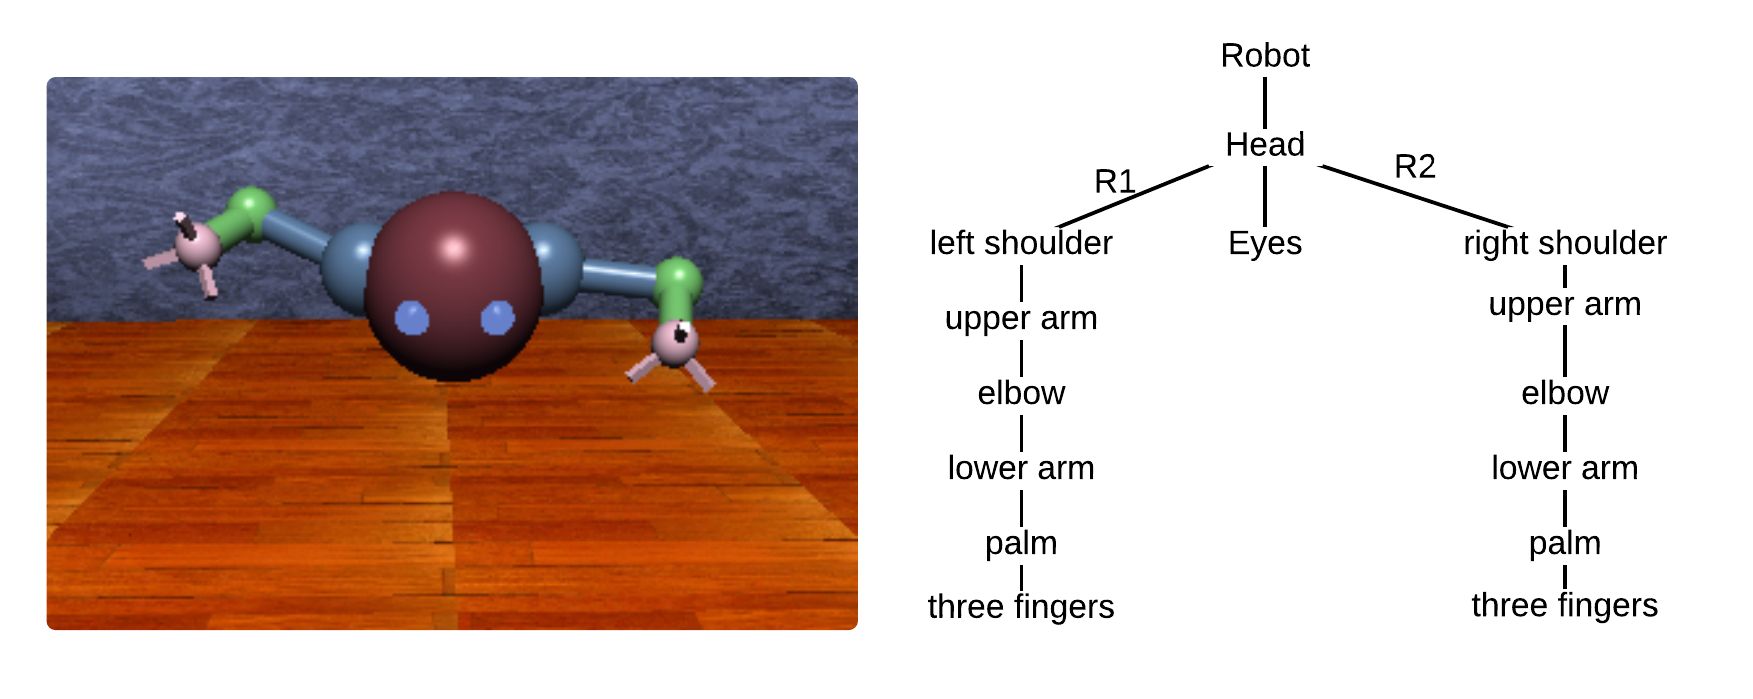
\includegraphics[width=12cm,height=5cm]{figures/scenegraph2.png}
\caption{A simple Robot and its scene graph after transformation.}
\label{fig:scenegraph2}
\end{figure}
Scene graphs can also combine bounding volume hierarchies, spatial
partitioning and many other techniques. There are also a lot commercial
software and 3D graphics libraries that use a scene graph such as Unity 3D and
Java 3D.
\section {Animation}
Animation could be divided into three categories: low-level, medium-level and high-level approach\cite{alan3D}. In the low-level approach, a geometric description is given such as the position and orientation. A typical example is keyframe animation.  In the medium-level approach, an animator has to input some rules which could be borrowed from real life or exactly physical rules instead of inputing the details of the geometric description. Usually an animator could know the rough results but no details of how the animation could be in this kind animation. To get the exact results, an animator has to run the simulation and adjust the rules for lots of times. Procedural animation and physical animation could be fell into this category. The high-level approach is behavioral animation.\cite{animationSlides} It will be performed by the coeffect of the environment setup and the animation internal system. The action selection layer in \cite{steering} is an example. In sum, the advantages of lower level approach is that it has more control abilities than higher level approach, but it will need lots of mannual efforts and sometimes it is infeasible to be implemented.
 
\subsection{Keyframe Animation}
In key frame animation, first the attributes of an object such as orientation, the position and joint angles between the links are at set at certain instances. Then interpolation of these attributes between these instances will be done. For example, A sequence of robot movement could be seen in figure \ref{fig:movingRobot}. Here for example first we set the attributes of the robot in \ref{fig:movingRobot-a}. Then also set the attributes of the robot in figure \ref{fig:movingRobot-d}. Then the interpolation of the position of the robot is a half circle linearly in x time. The interpolation of the orientation is 180 degree also in x time linearly. Then in-between pictures such as the pictures of figure \ref{fig:movingRobot-b} and figure \ref{fig:movingRobot-c} will be generated automatically. This idea was originated from Baecker's Genesys Computer Animation System in which the animator had to input
parameters of curves to specify both the path and timings of the 2D
animation \cite{keyframe1}. 
\begin{figure}
\centering
\subfloat[Part 1][]{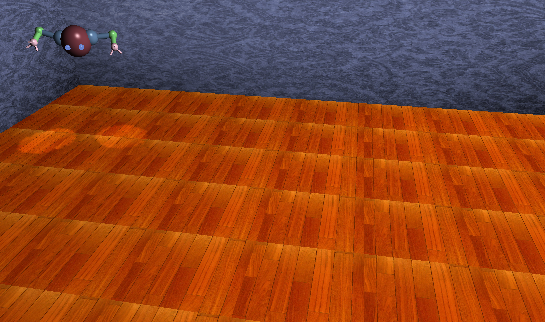
\includegraphics[width=2.5in,height=1.5in]{figures/rb1.png} \label{fig:movingRobot-a}}
\subfloat[Part 2][]{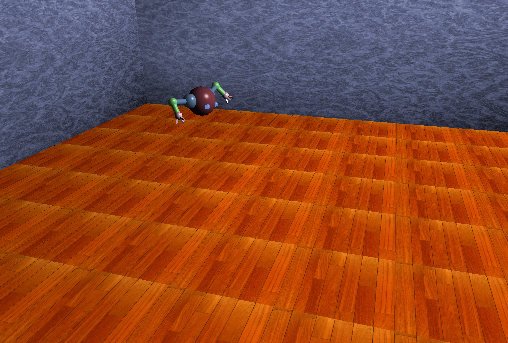
\includegraphics[width=2.5in,height=1.5in]{figures/rb2.png} \label{fig:movingRobot-b}}\\
\subfloat[Part 3][]{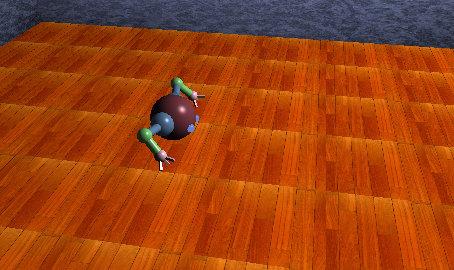
\includegraphics[width=2.5in,height=1.5in]{figures/rb3.png} \label{fig:movingRobot-c}}
\subfloat[Part 4][]{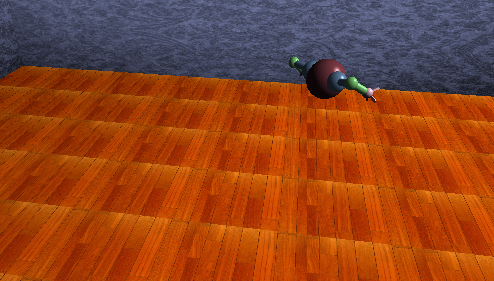
\includegraphics[width=2.5in,height=1.5in]{figures/rb4.png} \label{fig:movingRobot-d}}
\caption{A moving robot.}
\label{fig:movingRobot}
\end{figure}
Except these attributes, the shape can also be interpolated shown in figure \ref{fig:cows}. It is obvious that the number of the vertices of different pictures are different. One issue in shape interpolation is to tackle the relationship of corresponding vertices when the number is changing. The relevant research could be found in \cite{2d_shape}. 
\begin{figure}[ht!]
\centering
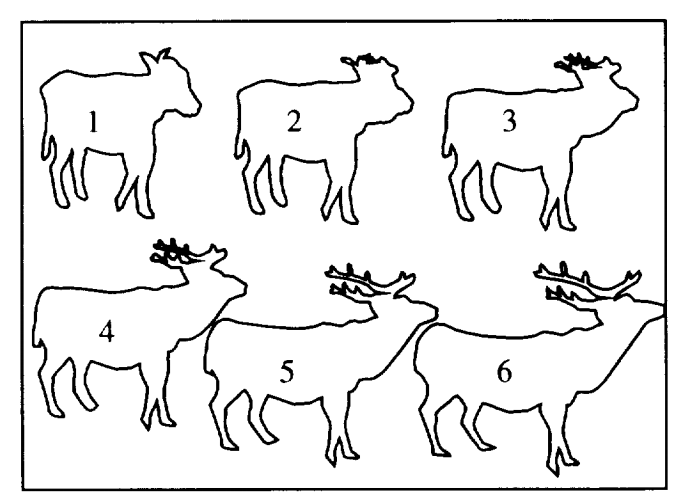
\includegraphics[height=8cm]{figures/cows.png}
\caption{Shape interpolation of a cow.\protect\cite{2d_shape}}
\label{fig:cows}
\end{figure}
Recent research combines the
data driven approach solves this problem \cite{keyframe2}, \cite{keyframe3}.  However, due to the
essence of the keyframe animation, even with data driven approaches
can not produce very substantial and dextrous animation for small
objects with an acceptable amount of data. Additionally, although \cite{keyframe4}
had implemented a system for capturing the motion data of insects, it
has several limits such as the system can only capture data from
planar geometry and only locomotion data is captured. Even if these problems are tackled someway, it is still has two drawbacks: production cost and lack of controllability. The problem lies in the traditional keyframe animation
is that the realism of the final motion heavily depends on the
knowledge and skills of the animator\cite{vince3D}. 
\subsection{Procedural animation}
Procedural animation refers to generation of motion based on procedures usually a set of rules other than pre-recorded data. Similar to keyframe animation, the procedural also has initial values and formulas to control how these values will be changed. But the difference is that in keyframe animation the initial values are specific attributes to show how the object is presented in an animation and the formula is about interpolation. While in procedural animation, the initial values contain some abstract attributes such as velocity and the formula show how these abstract values are changed which could be the forces which alter the velocity. It is infeasible to get the specific attributes such as position, orientation of an object in procedural animation. Examples of this kind animation could be seen in particle systems, plant growth, waterscapes, etc \cite{vince3D}.
Figure \ref{fig:mario} is a snapshot from the classic game Mario. It is a very simple form of procedural animation. When a key is pressed, acceleration is added to the velocity where the direction is the same as the key pressed. In this example, the procedure is a combination of responsive effects which is to add the acceleration in the same direction as the key pressed and deceleration in the reverse direction of the velocity. 
\begin{figure}[ht!]
\centering
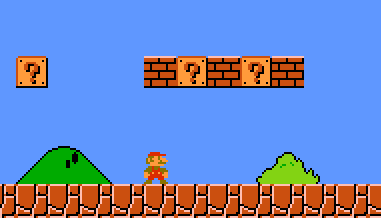
\includegraphics[height=6cm]{figures/mario.png}
\caption{A snapshot from classic game SuperMario}
\label{fig:mario}
\end{figure}
 Procedural animation is also widely developed is procedural
locomotion.\cite{loco1} implemented an interactive hierarchical motion control
system by using inverse kinematics with optimal approaches which
generate human walking over uneven terrain in different
environments. \cite{loco2} reviewed three categories of human walking which
includes procedural methods based on knowledge-based kinematic
animation.
\subsection{Kinematic animation}
The kinematics originally comes from the robotics which is intended to solve the relation between the joint angles and end-effector 
of an articulated figure. There are two categories in kinematic animation: forward kinematics and inverse kinematics. The forward kinematics is given all the joint angles to calculate the end effector X. The inverse kinematics is given the end effector X to calculate all the joint angles which produces the position of the end effector X.\cite{alan3D}
\subsubsection{Forward Kinematics}
Forward kinematics could be seen as a special kind of scene graph. In the graph, every node except leaf node is specification about the angles of joints while the leaf node contains the information of the end effector X. Thus every time a joint angle changes, it propagates the effects to all its descendant joints. As a result, the effector X will change. The advantages of it than keyframe animation is that the animator does not have to think all the attributes of a frame. Instead the animator could focus on the relation between linked parts.
So for example, to animate a human walking in figure \ref{fig:leg}. The animator just need to think the starting point of the root node of the hierarchy and angles between linked parts from the top node of the scene graph which is the hip to the "end effector" which is the foot. The curve in the picture is the angle between two linked parts.
\begin{figure}[ht!]
\centering
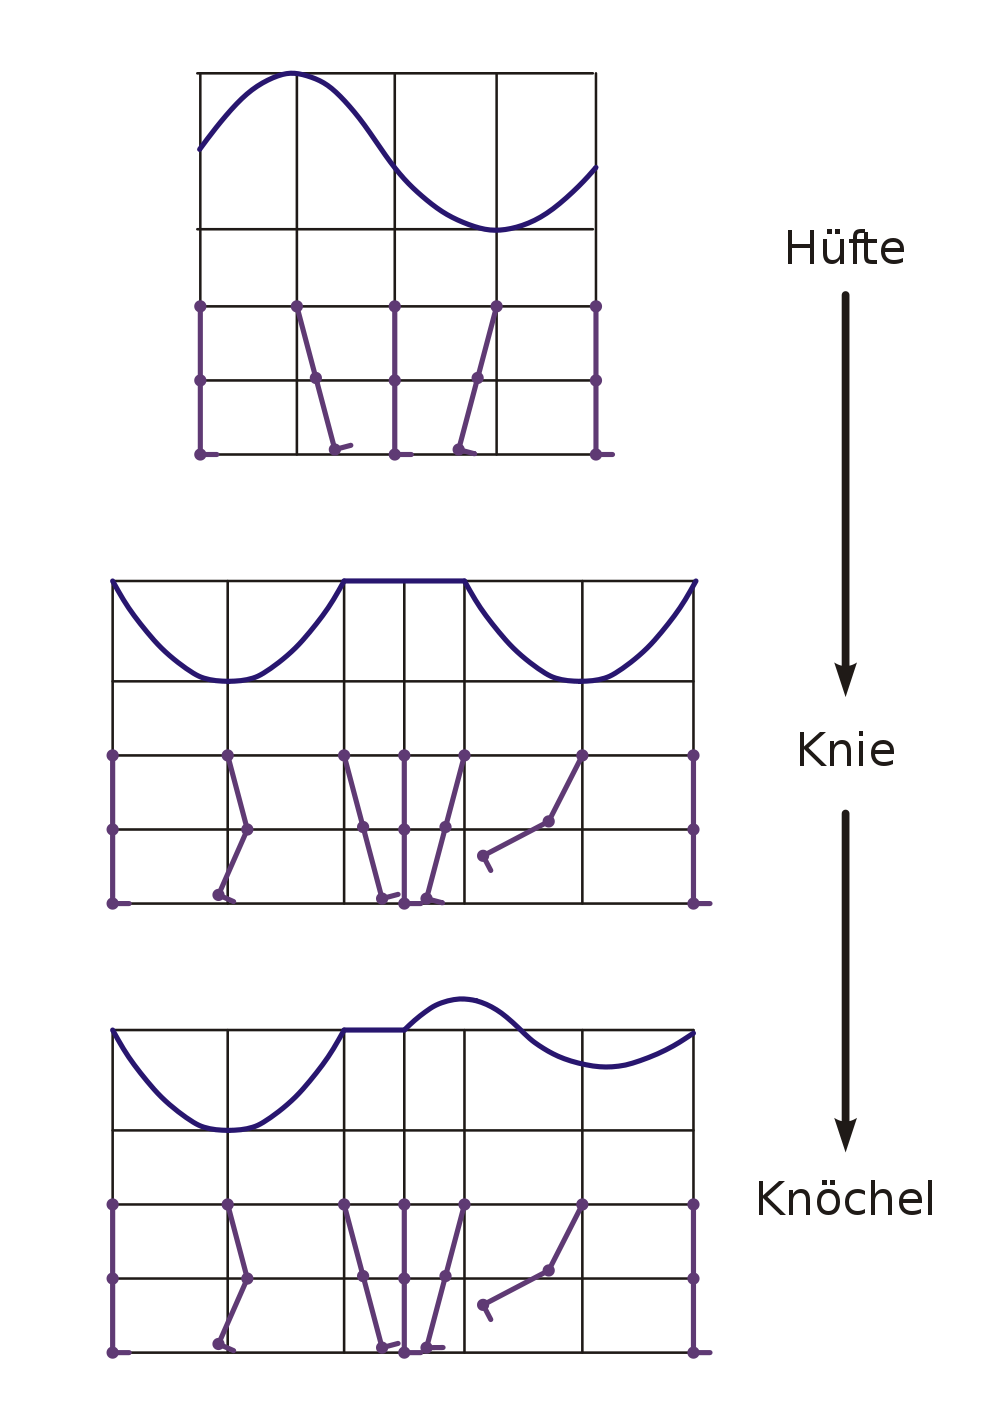
\includegraphics[width=12cm,height=5cm]{figures/leg_animation.png}
\caption{A human walking linked structure \protect\cite{leganima}}
\label{fig:leg}
\end{figure}
Since the structure could be considered as a scene graph or a hierarchy, the motion of the end
  effector is the accumulation of all the transformations that lead
  from the top of the scene graph to the "end effector"\cite{alan3D}. Given the state
  vector $\Theta{}$ which is the set of all the angles between different links in the link structure,
  the state vector $\Theta{}$ could be represented as\cite{alan3D}:
  \begin{equation}
  \Theta{}=(\theta_1,...,\theta_n)  
  \end{equation}
Because the object is a linked rigid structure which means given the starting point of the root node, each part of the structure including the end effector could be calculated by the state vector. Thus the position of the end effector \textbf{X} could be represented as\cite{alan3D}:
\begin{equation}
\mathbf{X} = f(\Theta)        
\end{equation}
So for example in a two link structure as shown in figure \ref{fig:twolink} , the end effector position is\cite{alan3D}:
\begin{equation}
\label{eq:1}
\mathbf{X}=(l_1\cos\theta_1+l_2\cos(\theta_1+\theta_2),l_1\sin\theta_1+l_2\sin(\theta_1+\theta_2))  
\end{equation}
\begin{figure}[ht!]
\centering
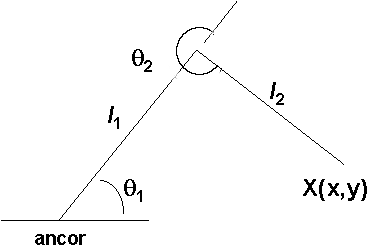
\includegraphics[height=5 cm]{figures/twolink.png}
\caption{A two link structure \protect\cite{linkpic}}
\label{fig:twolink}
\end{figure}
From the example, it is easily seen that it is more convenient than key frame animation. And constraints of angles between links could also be easily embedded. However, it is tedious to make the animation natural or as planned. Because the animator usually need to set the parameters from the top hierarchy to the bottom. If the link structures are complex, it is hard to make the end effector in the trajectory as planned\cite{alan3D}. This problem could be solved by inverse kinematics.
\subsubsection{Inverse Kinematics}
Inverse kinematics is the reverse of the forward kinematics. Unlike the forward kinematics tackle the animation problem from the top of the hierarchy to the bottom. It will first focus on the bottom of the hierarchy which is the end effector. So given the end effector X, all the parameters should be set explicitly in forward kinematics could be calculated by inverse kinematics\cite{Reference2}. Thus the problem could be summarized in an equation where given the end effector position\textbf{X}, calculate the state vector $\Theta{}$\cite{alan3D}:
\begin{equation}
\label{eq:2}
\Theta{}= f'(\mathbf{X})    
\end{equation}
Since the equation \ref{eq:2} is not linear and if the link structure become complex, it is very hard to invert the function. One way to solve the inverse kinematics is to linearise the problem by using Jacobian.\cite{alan3D}
\subsubsection{Jacobian}
Given $\mathbf{X}= f(\Theta)$ where $\mathbf{X}$ is of dimension n and $\Theta{}$ is of dimension m, the
Jacobian is the $n * m$ matrix of partial derivatives relating
differential changes of $\Theta$($d\Theta{}$) to differential
changes in $\mathbf{X}$ ($dx$), that is\cite{alan3D}:\\
\begin{equation}
dx/d\Theta=J(\Theta)\\
\end{equation}
By inverting the function, we get the following linear equation\cite{alan3D}:
\begin{equation}
\label{eq:3}
d\Theta=J^{-1}(\Theta)(dx) 
\end{equation}
Here iteration could be used by adding small changes dx towards the target position until the goal is reached. 
So one possible way to solve the inverse kinematics by using Jacobian could be\cite{alan3D}:
\begin{algorithm}
\begin{algorithmic} 
\REPEAT 
\STATE $dx \leftarrow$ small movement in the direction of $x$
\STATE $d\Theta \leftarrow J^{-1}(\Theta)(dx)$
\STATE $x=f(\Theta+d\Theta)$
\STATE $J \leftarrow dx/d\Theta$
\STATE $invert J$
\STATE $x \leftarrow x+dx$
\UNTIL{goal is reached}
\end{algorithmic}
\end{algorithm}
However since the equation \ref{eq:3} is an approximate way to calculate the real $\Theta$. As a result, the $dx$ in the algorithm above is not exactly the real changes of the end effector. The difference could be calculated by:
\begin{equation}
\|J(d\theta)-dx\|
\end{equation}
There are also several constraints in this approach. For example, differentiation is hard for a structure with many links. and the Jacobian may not invertible\cite{alan3D}.
\subsection{Dynamics and Physics-based animation}
In dynamic simulation, objects are modeled as masses acting under
forces and torques. The motion is produced through Newtonian
mechanics. Object motion in dynamic simulation is usually resulted
from a combination of automatic physical simulation (e.g., failing due
to gravity or floating in water due to buoyancy) and user suggested
forces (apply torque so that a moving car changes its velocity
direction) \cite{dy1}. It is an effective means to produce complex and
realistic behavior that will be impractical for kinematic
approaches. However the shortcoming of this approach is hard to
produce natural looking animation \cite{dy2}. 
There are two major approaches in physics-based animation. One is
motion synthesis approach which is similar to the combination of
inverse dynamics and kinematics. The difference is that it also takes
account of the limitations of the muscles. The main task of this
approach is to derive suitable actuator control functions which is
difficult when the muscle model is complex. The other approach is
constraint-based approach which involves constrained optimization and
inverse dynamics. 


\section{Arthropod Simulation} % (fold)
\label{sec:arthropod_simulation}

% section arthropod_simulation (end)
An early research on arthropod simulation could be seen in \cite{arsimu1} where a
forward dynamic simulation algorithm was proposed for the coordination
of the locomotion of six-legged figure. The system has three main
procedural components: a dynamic simulator, a gait controller and
motor programs. The dynamic simulator is based on Featherstone's
Articulated Body method which uses reduced coordinates to represent
motion in a computational time linearly proportional time with N being
the numbers of degrees of freedom. The gait controller is based on five rules of
the gait behavior of many insects proposed by Wilson\cite{arsimu2}: 
\say{
\begin{enumerate}
\item A wave of protractions (forward movements of the legs relative to
the body) runs from posterior to anterior (and no leg protracts until
the one behind is placed in a supporting position). 
\item Contralateral legs of the same segment alternate in phase. 
\item Protraction time is constant.
\item Frequency varies (retraction time decreases as frequency increases). 
\item The intervals between steps of the hind leg and middle leg and between
the middle leg and foreleg are constant, while the interval between the
foreleg and hind leg steps varies inversely with frequency. 
\end{enumerate}}

The motor system is composed of stepping program which compute forces
necessary to produce steps and deliver forces to legs to forward the body.


\cite{arsimu3} developed a system which is used to study insect
walking. The system describe a simple neural network called Walknet
which is a biologically inspired network to control six-legged
walking. Another research on insect walking study which focus on leg
searching movements can be seen \cite{arsimu6}.
Research on eight-legged arachnid and autonomous learning of
locomotion can be found in \cite{arsimu4}. They adopted a
physics-based approach at modeling and implement functions that drive the arachnid to move
at the minimum expense of energy.

An alternative approach can be found in \cite{arsimu5} which adopted the motion capture techniques to
synthesis the insect motion. The system used tracking techniques and a
3D point generating to capture the motion of the insects and developed a optimal path following approach.

\cite{thesis} adopted a novel approach, the core idea of which is instead of treating limbs as force source, it take the main body as the force source. Then the main body deliver the force to its limbs. The steps of the arthropod is triggered by the forces accepted from the main body. The idea is quite similar to inverse kinematics that given the end-effector main body, the exact posture of the legs is calculated except that the forces are also considered to regulate the speed and other constraints. The main components of the system is shown in figure \ref{fig:spider_module}. The black lines and yellow lines indicate passive and direct effects on the spider.
\begin{figure}[ht!]
\centering
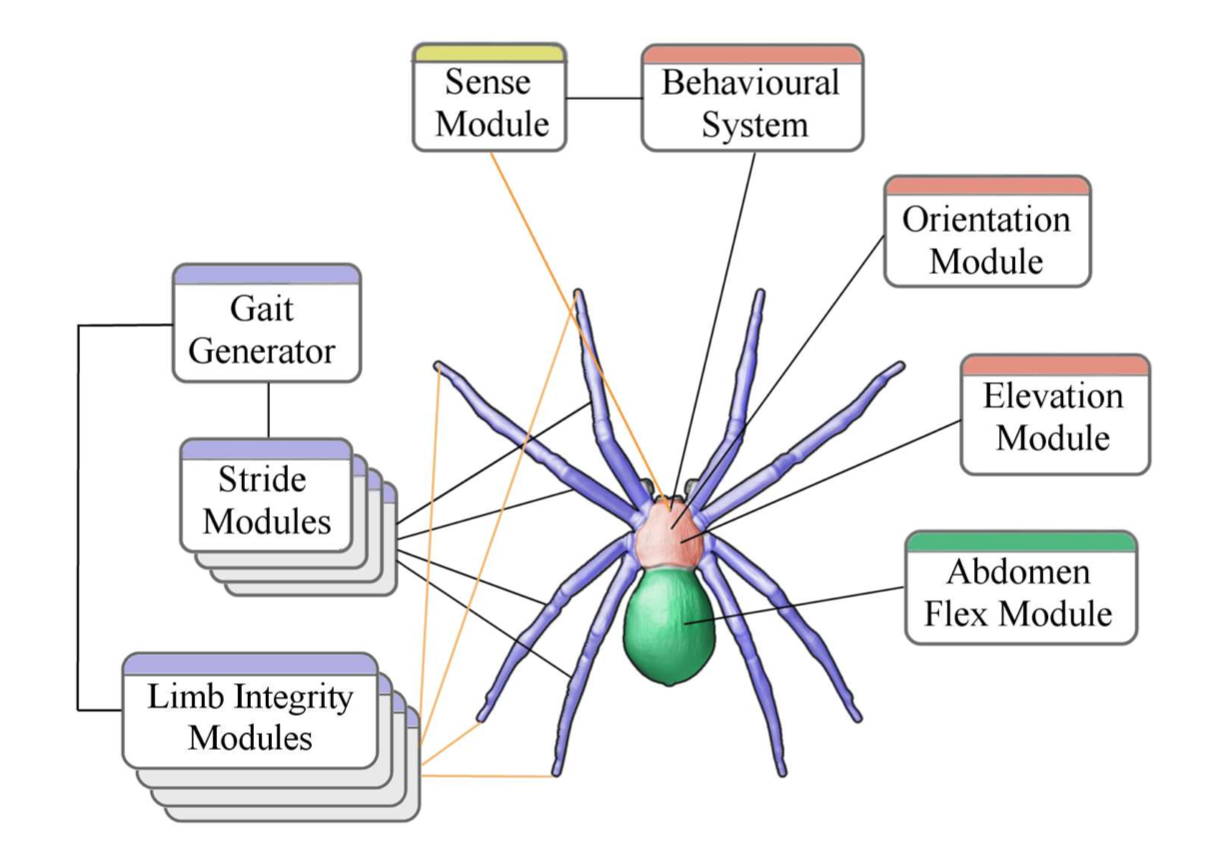
\includegraphics[height=8 cm]{figures/spider_module.png}
\caption{Main components of the arthropod animation system. \protect\cite{thesis}}
\label{fig:spider_module}
\end{figure}.
The schema of the system is based on the three locomotion layers which originally proposed in \cite{steering}. The three locomotion layers are action selection, steering and locomotion layer. The action selection is to choose which kind of behavior intend to animate which could be random stop, wander. The steering behavior is how the object move without consideration of the details of the locomotion. The locomotion layer is actually how to move the limbs given a specific steering behavior. 
\begin{figure}[ht!]
\centering
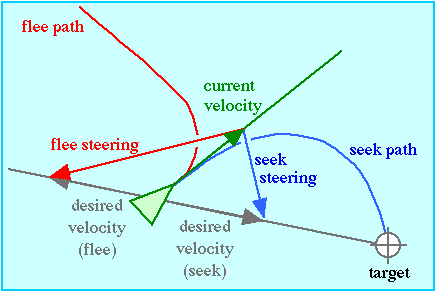
\includegraphics[height=6cm]{figures/seek.png}
\caption{Seek and flee steering diagram. \protect\cite{steeringImage}}
\label{fig:seek}
\end{figure}
The behavior system is corresponding to the action selection layer and the steering layer in \cite{steering}. An example of seek and flee action along with its steering details is shown in figure \ref{fig:seek}. The behavior system in \cite{thesis} mainly describes the kinematics of the spider without much consideration of limbs. Thus it introduce an abstract separation between the main body and limbs. The basics of the behavior system is meant to implement several behaviors such as wander, seek and flee by using physics and configuration which include such as the maximum speed of the spider, the maximum DOF of the joint between abdomen and thorax.
The rest of the system is mainly corresponding to the locomotion layer in \cite{steering}.
The major modules in the locomotion layer involve IK, stride module, limb regulatory modules, elevation and orientation module, abdominal flexing and the sense module. The examples of spider with IK is shown in \ref{fig:spiderIK}.
\begin{figure}[ht!]
\centering
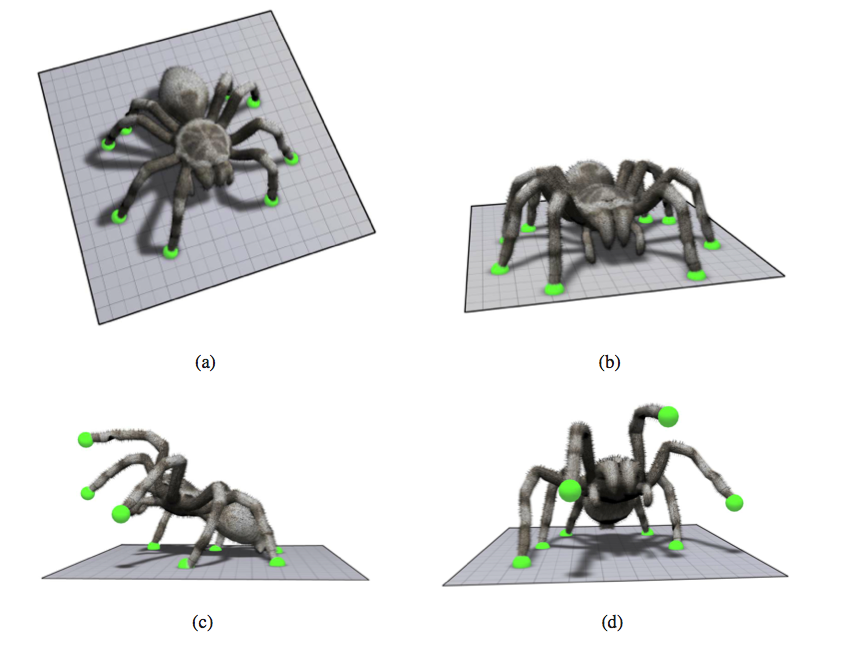
\includegraphics[height=10cm]{figures/spiderIK.png}
\caption{Results of spider with IK. \protect\cite{thesis}}
\label{fig:spiderIK}
\end{figure}
The main aim of the stride module is acting as a procedural step which move the creature's foot from initial to goal position. Results on the trajectory produced by the stride module is shown in figure \ref{fig:stride}.
\begin{figure}[ht!]
\centering
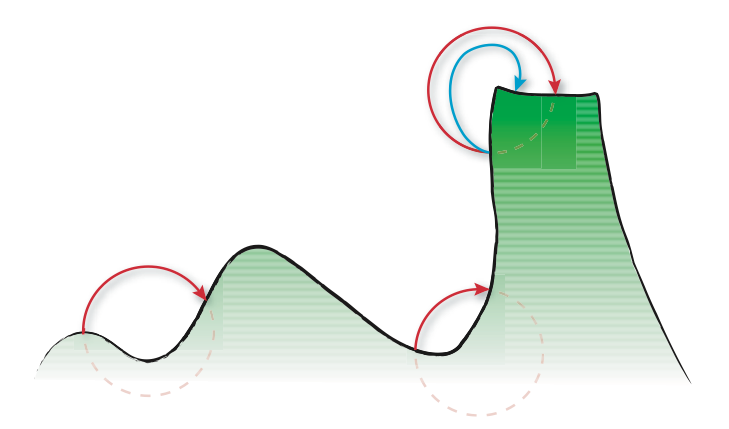
\includegraphics[height=6cm]{figures/stride.png}
\caption{Step path produced by the stride module. \protect\cite{thesis}}
\label{fig:stride}
\end{figure}
The limb regulatory modules act as an error checking function when an error in the limb is detected, the
gait generator will be invoked to correct a step. The gait pattern adopts the tripod trait. 
The purpose of the elevation and orientation modules is to control the absolute
orientation and the height of the main body which is the creature's
thorax and abdomen segments so that it conforms to a natural posture
relative to the position of the creature's feet. The function of abdominal flexing
is similar to limb regulatory module which is give constraints to the
joint which connects the thorax and the abdomen to make the posture
more natural. 
There are also two other modules. The sense module and the gravity activation.
The sense module acts as the eye of the creature which implemented mainly by the technique ray tracing but also take consideration of the limbs' feedback. The gravity module is added last to tackle the problem of special cases such as lose grip. The gravity activation is added last since it won't interfere the creature's normal locomotion since the mass of the creature is light and this choice will save lots of unnecessary constraints of the physical model\cite{thesis}.
\section{Arthropod Rendering}
The general technique to render an arthropod is texture mapping
which is a method for adding detail, surface texture or color to a 3D
model. For example, the surface of an arthropod could be added to the
mesh model to make the arthropod more realistic. Since the surface of the
arthropod is not smoothing, a bump mapping texture could be used to
show the indents in the surface. 
However, it is not enough. Because it is infeasible to use just
texture mapping to show the subtle detail of a
spider such as the fur of a spider. 
A common approach used is to use polygon strip fur which is produced
from side-view texture maps \cite{fur} as shown in figure \ref{fig:fur}.
\begin{figure}[ht!]
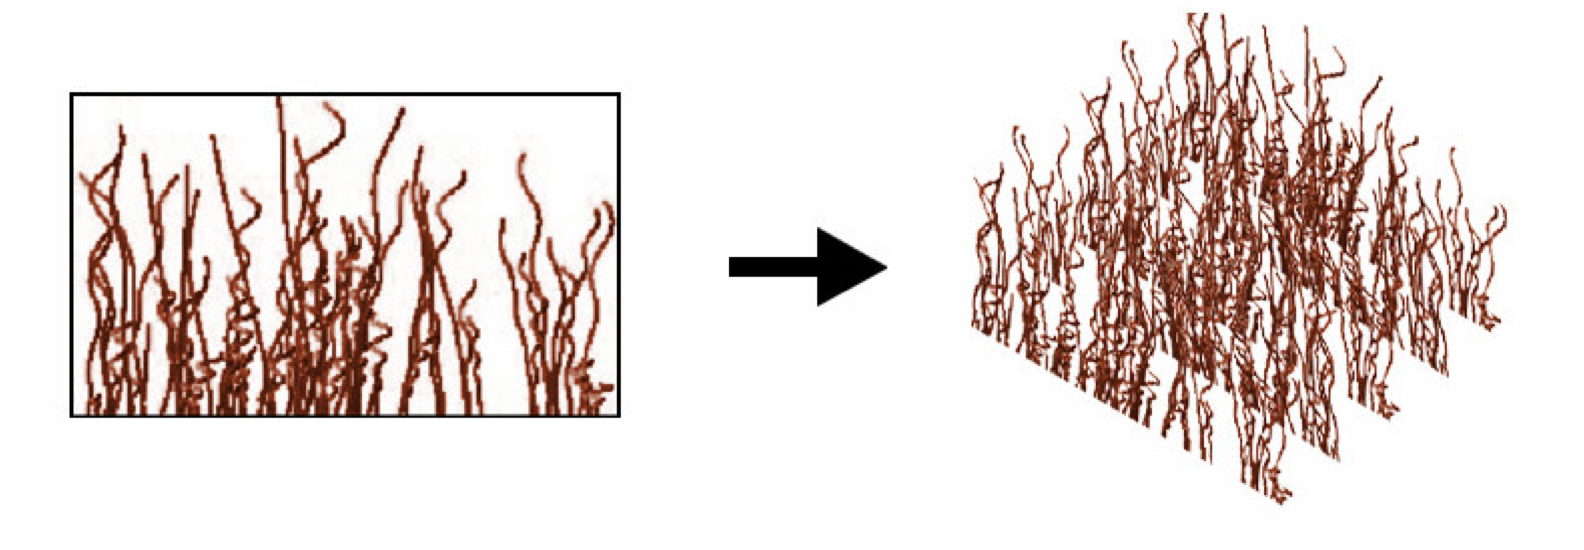
\includegraphics[height=5 cm]{figures/fur.png}
\caption{Polygon strip fur \protect\cite{fur}}
\label{fig:fur}
\end{figure}
The drawback of this approach is that if the fur is viewed from
side-view angle or directly above, it will not be rendered. However
this could be solved either in a 'cross-hatching' approach which is
strips are arranged at various angles across the skin surface or a
'Billboarding' approach which rotates any given polygon given strip to
always face to the camera \cite{fur}.
The most popular to generate fur
of an arthropod is the fins and shells approach. The fins technique 
involves the creation of textured polygon strips along the edges of
the base model and the fins extruded by default along the normal of
each edge \cite{thesis}.  The stages of fins application over a spider
is shown in \ref{fig:fins}.
\begin{figure}[ht!]
\centering
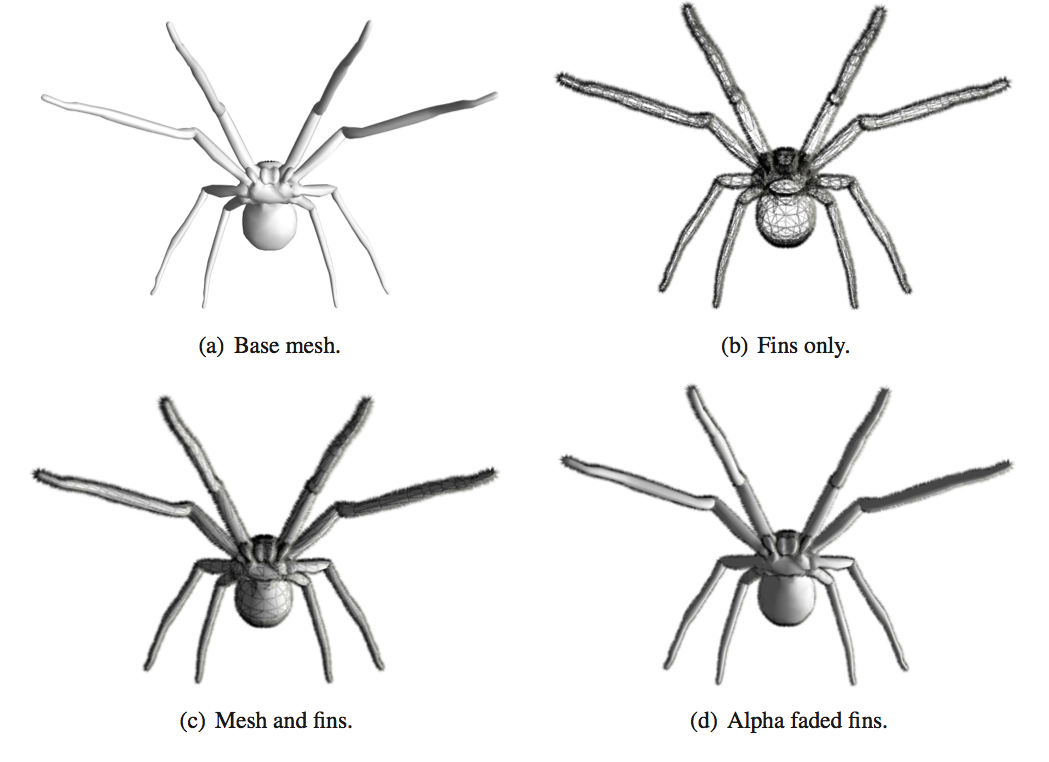
\includegraphics[height=12 cm]{figures/fins.png}
\caption{stages of fins \protect\cite{thesis}}
\label{fig:fins}
\end{figure}
The basic premise behind shells is adopting the texels approach with
traditional texturing methods to render a series of layers on which
cross-sections of a fur patch are rendered\cite{thesis}.
In sum, the polygon strip techniques could produce deserved
results. However there are drawbacks in it. The 'cross-hatching' will
result in slow rendering time for complex geometry. The bill boarding
approach does not have this problem but can not be viewed from
directly above. The fins and shells approach is usually more efficient
than polygon strip model and only major restriction is the maximum
DOF of the fur is 45$^\circ$ \cite{fur}.


\chapter{Requirement and Analysis}
This chapter is to analysis the possible solutions according to the aims of the project as well as evaluation criteria. In section 3.1, the problem is divided into 3 parts which are modeling the spider, spider animation and spider rendering. Due to the time constraints, the project will mainly focus on spider animation. Initially a simple rendering for the spider is sufficient for the project. The Oculus Rift is also briefly introduced in this section 3.5. Section 3.6 and 3.7 are requirements lists and how the project will be evaluated. The final section is about ethics and legal considerations of the project.
\section{Overview}
The main aim of the system is to develop realistic spider animation under Oculus Rift. There are two main aspects which are animation part and rendering part. For the animation, the procedural or rule-based method will be adopted. The basics of this part is to make the behavior follow the biology constraints which could include the maximum speed of the spider or the DOF of each joints. These could be tackled by observation of a real spider or knowledge from biology. The second part is to tackle the step behavior. This is the major part of the animation. The step patterns will be based on \cite{arsimu2} and implemented by inverse kinematics\cite{alan3D}. As a result of time constraints for the project, initially a simple rendering is sufficient for the project. Thus the analysis of the project could be divided into following sections: modeling the spider, spider animation and spider rendering.
\section{Modeling the spider}
As stated in chapter 2, initially polygon meshes will be adopted to represent a spider which is shown in figure \ref{fig:spiderMesh}. The initial spider polygon mesh will be adopted from others' work.
\begin{figure}[ht!]
\centering
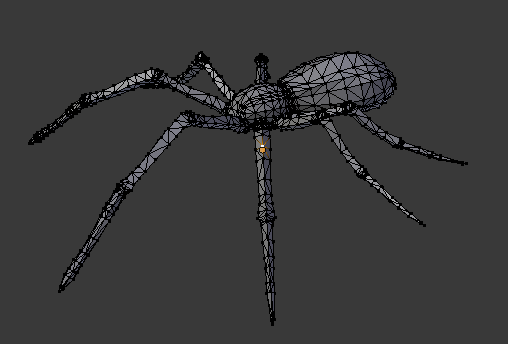
\includegraphics[height=6 cm]{figures/spiderMesh.png}
\caption{A simple spider mesh model. \protect\cite{spiderMesh}}
\label{fig:spiderMesh}
\end{figure}
There are two general methods to manipulate polygon meshes of articulated creature such as the spider. The first approach is to use a pure scene graph approach. But there are three main problems: first problem is how to represent a node in a scene graph. In the previous simple robot example, since the components of robot are all primitive graphics such as sphere and cylinder, the axis could be considered as an abstraction to represent a node. However for a more complex polygon meshes model such as spider shown in figure \ref{fig:spiderMesh}, since the edges of components are irregular, it is hard to find some abstraction layer to represent a node. The other two problems are vertices are changing in local coordinate system and hard to estimate the real outcome of the animation. As a result the project will adopt skeletal modeling, rigging and skinning should be done. 
Most modeling software such as 3DMax, Blender has the function of automatic rigging. However, it is most for human figures. So in this stage, the rigging and skinning of the spider will be done manually by using Blender. An example of spider rigging done manually by using Blender can be seen in figure \ref{fig:spiderRigging}.
 \begin{figure}[ht!]
\centering
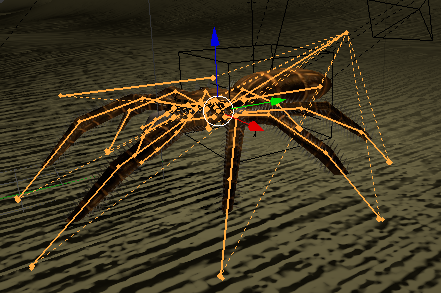
\includegraphics[height=6 cm]{figures/spiderRigging.png}
\caption{A rigging spider example. \protect\cite{spiderModel}}
\label{fig:spiderRigging}
\end{figure}
Also in this stage, a configuration file about biological modeling which mainly covers the limitations of a real creature such as DOF of all joints and speed limitations will be made. The data will be adopted from biology or observations of the natural extent of the spider posture.
\section{Spider animation}
The realism of the spider animation depends on two aspects: First, it should have some different behavior patterns to show its intelligence. Here behavior patterns could be wander, seek food, jump. Secondly, the details of how it take a step.
The three layers of locomotions from \cite{steering} provides a main scheme for this project. The three layers of locomotion is action selection, steering behavior and locomotion behavior. \cite{thesis} implemented the arthropod simulation also on the schema but used a hybrid approach of procedural and physically based animation. The steering behavior in \cite{thesis} acts as a middle layer of delivering forces according what the action selection is and also maintain the overall kinematics of the spider. The difference between \cite{thesis} and this project is instead of considering how the forces are delivered, the project will considering maintain relation table which deals with the relations between the action selection and rules will applied to the spider. Here rules mainly deals with the kinematics. In sum, the three layers design provides the solution of how to show the intelligence of the spider and a scheme of the animation part of the project.
Since the first layer which is the action selection layer is intended to solve the problem of intelligence of the spider. There are two subtasks in it. The first is to define a table which maintains the relation between action selection and pace. A normal spider pace pattern description could be seen in \cite{arsimu2}. A similar pattern which is usually used as normal hexapod gait is shown in figure \ref{fig:triGait}.
 \begin{figure}[ht!]
\centering
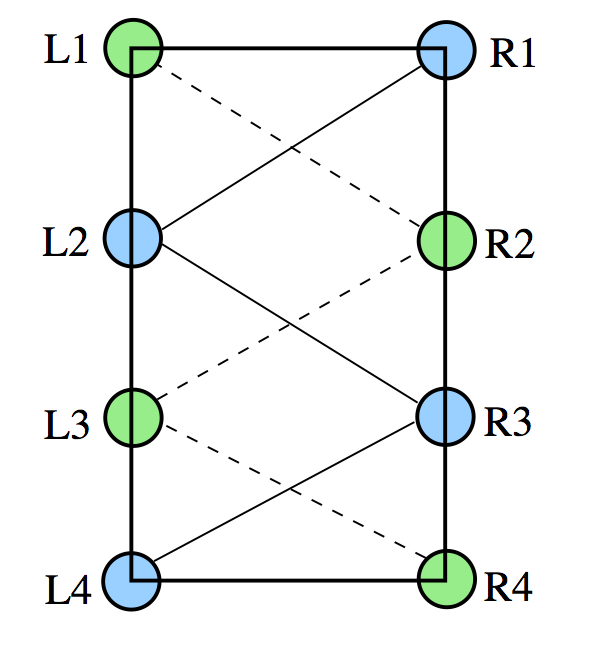
\includegraphics[height=6 cm]{figures/triGait.png}
\caption{The Tripod Gait. \protect\cite{thesis}}
\label{fig:triGait}
\end{figure}
A simple implementation of using the tripod gait shown in \ref{fig:triGait} could be lifting up the limbs in the same color at the same time. Limbs in different color are stepping in turns. However in reality, usually the limbs in the same color are not exactly at the same time. For example, when the limb L1 lift up a bit, then the limb R2 begun lifting. So the timing of how each limb lift up is very important. Figure \ref{fig:gaitTiming} is the timing strategy adopted by \cite{thesis}. The limbs in the different color are corresponding to the gait pattern in figure \ref{fig:triGait}.
 \begin{figure}[ht!]
\centering
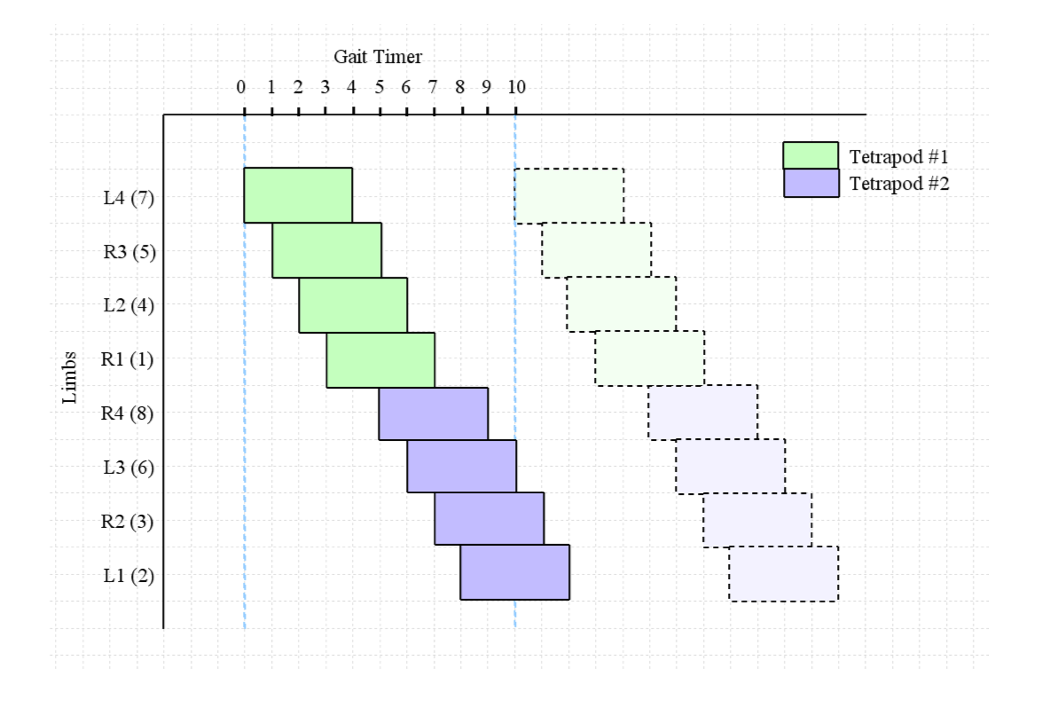
\includegraphics[height=6 cm]{figures/timing.png}
\caption{The Gait Timing. \protect\cite{thesis}}
\label{fig:gaitTiming}
\end{figure}
But the pattern of the steps will not fit with the behavior such as explore or wander. When the spider explore, the spider may use the front limbs to detect the front places to check whether the terrain is uneven or is there a wall before it. The gait pattern may be keep waving the two front limbs, other limbs are moving backward and forwards a bit. While when the spider wander, the heading may change frequently, so one side of the limbs may step more frequently than the other side. The seeking food behavior may be dependent the extent of hunger of the spider, if the spider is a little hunger, it may step more frequent. But when it suddenly find a food near it, it may just directly jump. And if the spider is very hungry, it may not have strength, so it will step very slowly and even without lifting some limbs. The picture could be like a spider use some of its legs to drag the whole body. But due to the fact that it is very hard to estimate the difficulty of implementation. The project first will add the basic behavior such as simple walk, jump and climb walls. If time allowed, behaviors mentioned above will be added to the project. 
A sense module also need to be built because a sense module could solve some action such as seek food or walk on a ball surface\cite{thesis}. It should have two parts which are the foot detection and the ability to see. The second layer is the steering layer which mainly deals with the velocity of the spider according to which action is selected. Though forces will not be considered in the project, acceleration is still needed to be considered. The basics of implementation may be similar to the game SuperMario mentioned in chapter 2. The difference is the acceleration will not triggered by the player but by the coeffect of the environment and the current behavior pattern.  
The last part is to solve how the steering behavior could fit with the pace pattern proposed above. The major part of this stage is mainly to use inverse kinematics with the pattern of the steps. Two approaches which could solve the inverse kinematics are Cyclic Coordinate Descent and Jacobian Transpose.
\section{Spider rendering}
As stated before, the main task of spider rendering is mostly to render the details of the spider. There are three main approaches to render fur which are polygon strip approach, texels approach and shells approach\cite{fur}. The polygon strip approach is easier than the other two approaches. The texels approach is the one which could best results but resource demanding. The shells approach take the concept of the texels approach but implemented the same idea with traditional texture mapping approaches\cite{fur}. The first and third approach are two most popular approaches to render the fur of the spider. Apart from the fur, there are also other aspects could be considered such as using bump mapping to show indents or using soft shadows to make the spider more real. But as stated before, the project will use a very basic rendering which maybe just setting the material property without using texture at all. If time allowed, techniques mentioned in this chapter will be considered.
\section{Oculus Rift}
The Oculus Rift is a virtual reality headset developed by Oculus VR. It enables users to seamlessly look around the virtual world. It tracked every little movement of users' head to create a natural experience. Further more, it provides a stretching world view instead the traditional way which limited users' eyes in a boxed screen.\cite{rift1}
It publishes its SDK which could be integrated ether into OpenGL or Unity3D. Due to the easy setup of Oculus Rift with Unity3D by plugins, the project will choose Unity3D as the main developing software.
\section{Requirements Lists}
\begin{itemize}
  \item \textbf{Extensibility}  
The project should provide a configuration file which could be easily altered by non-programmers to change the details of spider animation which include the basics of animation such as the DOF of the joint between the abdomen and thorax, the max speed of the spider and the details of the intelligent behavior which may be the scope of area of the eyes of the spider.
 \item \textbf{Basic Animation} 
  The spider should have abilities to walk on flat surface and a sphere surface. The spider should have basic behaviors: climb walls and jump. If no advanced behavior is triggered and there is no any user input, the spider will fall into default mode in which a spider will explore the areas in these basic animations.
\item \textbf{Advanced behaviors}
  The spider should have at least one advanced behavior mentioned in section 3.3 such as seek food. When the advanced behavior is triggered, the way the spider moves such as the stepping pattern and speed will change accordingly; for example, if the user throw a piece of food within the spider's view, the spider will jump or run to the food. However, the advanced behaviors will be determined by the progress of the project which means the final advanced behavior may not contain the seek food but will contain at least one mentioned in section 3.3.
 \item \textbf{User Control}
 In order to observe the animation conveniently, user interface will be implemented to handle following functions:
 \begin{itemize}
  \item ability to zoom or change the position and orientation of the camera.
  \item ability to trigger the advanced behaviors of the spider
  \item ability to control the spider(e.g. move and jump)
 \end{itemize}
\end{itemize}
\section{Testing and Evaluation}
\subsection{Testing}
It is hard to predict the final results and approaches adopted in the final project for lack of experience in relevant projects. The main development method adopted is agile software development. Prototype of the project meeting part of requirements will be implemented very quick. As a result, the testing phase will be embedded in different phase of the development and black-box testing will be used. 
In black-box testing, the expected output is the actual image of the spider of animation of the spider. The input are methods adopted or parameters which affect the animation. Since there may be lots of changes in the project, testing will be mainly integration and system testing. 
\subsection{Evaluation}
\begin{itemize}
  \item \textbf{Extensibility}  
   The extensibility mainly focus on the configuration file. The ease of use and how many parameters that can be altered to change the animation could be evaluated. The ease of use means the file should be well organized and has no ambiguities. The parameters could be DOF of each joint, speed, the view scope of the spiders, etc.
  \item \textbf{Realism} 
Two main approaches are proposed to judge the realism of the animation. One is to judge the realism by users based on their memories of spider movement. The other is to compare the animation with real video.
\item \textbf{Rendering}
Though the rendering is not required in the project, if rendering techniques other than the smooth rendering adopted, it should be considered as a bonus to the project. 
\end{itemize}
\section{Ethics and Legal considerations}
One big problem of using Oculus Rift is causing motion sickness\cite{motionSick}. It is common in first-person shooter video game such as Counter-Strike. So the users should be warned about the motion sickness issues before he wears the Oculus Rift device. Also because by using Oculus Rift, the user is so deeply immersed in the virtual reality that he may not pay attention to real environment. For example, he may want to step back when a spider comes close to him which may cause injury. So a third person should be around the users who use the device. 
There is another issue about the fear of spiders. A banner or sign should be placed in obvious places to indicate the issues and in the meantime the users should be notified about all the issues above verbally.
According to the guides and code in \cite{ushuman}\cite{ukhuman}\cite{humanPro}, human participants should be informed the risks of the experiment, the values of the experiment and sign a form of written informed consent or parental permission. However due to the fact that most cases involving human participants are usually medical or psychological and the project does not have the same extent level of risks. For the project, all the risks mentioned above along with the usage of project should be stated clear in a print form documentation, and need users to sign the form before use the Oculus Rift device.

\chapter{Planning}
\section{Risk analysis}
There are several risks in the project. The first risk is hard to estimate the time of the model and rigging due to lack of relevant experience. So initially to tackle this problem, a spider model will be found on the Internet. The biggest risk is to implement the three layers in\cite{steering} which is usually implemented under the physical modeling. The second biggest risk is the inverse kinematics may not produce the expected results or is hard to be embedded in the system due to lack of experience. The fall-back schema is to implement a behavior-stepping pairs instead of implementing the three layers. About the animation techniques, if the expected results or the skeleton animation is too hard to implement, scene graph techniques along with procedural animation or keyframe animation will be adopted. The results of adopting backup plan is that the animation results will not be good as expected and as a result of changing plan, some requirements listed in Chapter 3 may not be fully satisfied.
There are also risks that there not enough volunteers to judge the project. Two possible solutions to it is that invite the volunteers before the poster session and evaluate the project against videos of real spider which does not require many volunteers. 
If the results of the project are not ready on time for the evaluation stage, efforts in the project should be ready to be demonstrated either under Oculus Rift or using a PC. As a result, work in each stages should be recorded to prepare for this kind risk. 
There are also some risks which can not be foreseen at this stage. So contingency time along with some risks mentioned above should be considered in project plan.
\section{Project plan}
The project plan is based on the analysis in Chapter 3. Figure \ref{fig:gantTable} and figure \ref{fig:gant} are Gantt table and chart. 
\begin{figure}[ht!]
\centering
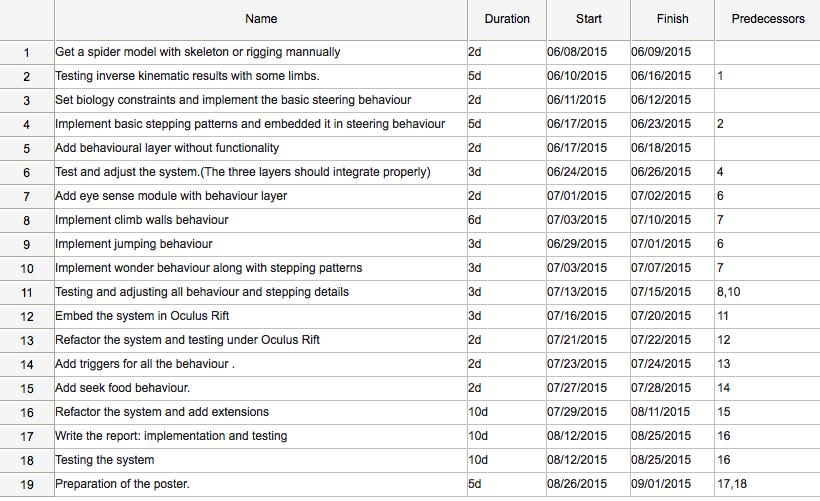
\includegraphics[width=15cm]{figures/gantTable.png}
\caption{Gantt Table}
\label{fig:gantTable}
\end{figure}
\begin{figure}[ht!]
\centering
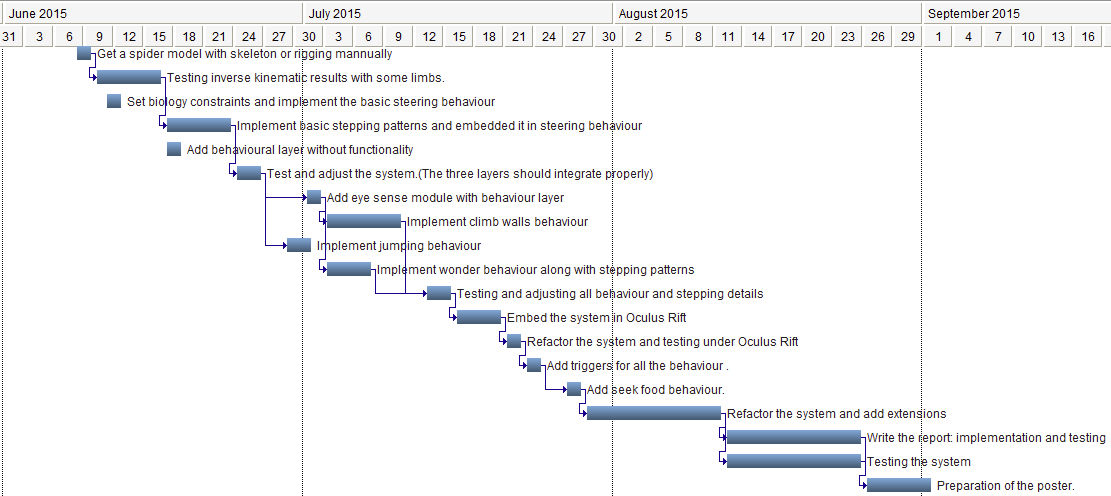
\includegraphics[width=15cm]{figures/gant.png}
\caption{Gantt Chart}
\label{fig:gant}
\end{figure}
All tasks in the figure are assigned more time than the amount that they can be finished in. About the animation techniques may be different than as planned, the task 2 "Testing inverse kinematics..." is testing whether the technique is suitable. So the animation technique could be chosen properly in the early stage and the techniques will not interfere with the following tasks. About the risk that the main schema may not work, the plan is added system prototype testing and adjusting stage. Besides, the system will not implement the main schema such as three layers in \cite{steering} at early stage, it will implement several subtasks which is not dependent on the main schema. The main schema will be added in later stage to avoid much dependancy. 

\chapter{Conclusions}
Previous research and techniques relevant to the project were reviewed. In this part, some general animation techniques were briefly introduced. These include keyframe animation, procedural animation, kinematic animation and physical animation. The fundamentals of animation such as how to represent an object, animation control techniques and rendering were also included. Knowledge specifically for simulating an arthropod includes some biology knowledge, algorithms for simulating steps or paths and some possible implementations.
Analysis on possible solutions were given based on research of previous work. Project requirements, evaluation criteria were also set.  Planning including risk analysis and Gantt Chart was made after it.


The future work will mainly follow the Gantt Chart in the planning section. However, details may be changed due to risk of technical issues or time. The future work is generally described in figure \ref{fig:fw}. The work will be circulated until all the techniques were tested and embedded into the final system. The techniques testing mainly refers to implementation of a demo with a specific technique to be used in the project. The techniques testing is required because the techniques may be very hard to implement or cannot produce expected results. The merge phase mainly refer to integrate new module to the project. The documentation will be written after the whole project. 
\begin{figure}[ht!]
\centering
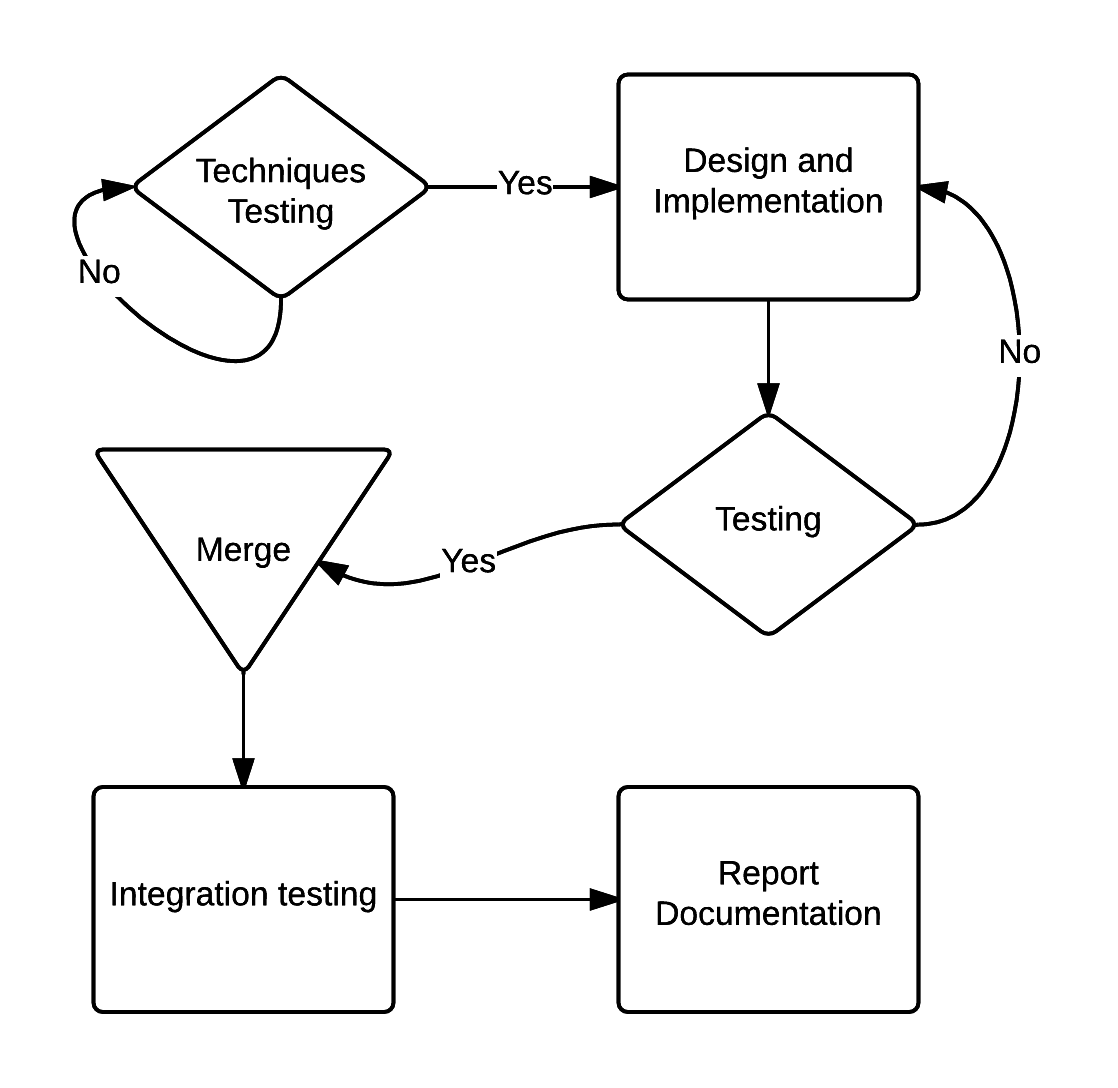
\includegraphics[width=10cm]{figures/fw.png}
\caption{Future work}
\label{fig:fw}
\end{figure}


\bibliographystyle{acm} 
\bibliography{mybibliography} 

\begin{appendices}
\chapter{An appendix of some kind}


\chapter{Another appendix}


\end{appendices}

\end{document}

%%% Local Variables:
%%% mode: latex
%%% TeX-master: t
%%% End:
